\documentclass[10pt,a4paper]{article}
\usepackage[utf8]{inputenc}
\usepackage{amsmath}
\usepackage{amsfonts}
\usepackage{amssymb}
\usepackage{hyperref}
\usepackage{listings}
\usepackage[many]{tcolorbox}
\tcbuselibrary{listings}

\newtcblisting{mylisting}{
  listing only,
  hbox,
  colframe=cyan,
  colback=cyan!10,
  listing options={
    language=Fortran,
    basicstyle=\small\ttfamily,
    breaklines=true,
    columns=fullflexible
  },
}

%hyperlink parameters
\hypersetup{
    colorlinks=true,
    linkcolor=blue,
    filecolor=magenta,      
    urlcolor=cyan,
    pdftitle={Overleaf Example},
    pdfpagemode=FullScreen,
    }
\urlstyle{same}

% Code style font
\usepackage{xcolor}
\definecolor{light-gray}{gray}{0.95}
\newcommand{\code}[1]{\colorbox{light-gray}{\texttt{#1}}}
%\newcommand{\code}{\texttt}

% Fortran source code style



\author{Sarah}
\title{OpenACC using Colab}
%\date{today}

\begin{document}
\maketitle{}
\newpage

\section{Part 1: Introduction}
This document offers an introduction to porting algorithms on GPU with OpenACC using Colab.\\

\section{Part 2: Running a Fortran code in Colab}
\subsection{About Colab}
Colab is a free cloud service proposed by Google based on the Web Open Source application Jupyter-Notebook.\\
\subsubsection{Environment}
Here, we work exclusively with Fortran source code. In Colab, we can see that the GNU Fortran Compiler (gfortran) is already installed and we can check which version is available:
\begin{center}
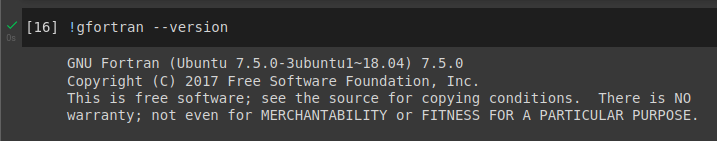
\includegraphics[scale=0.5]{fortran_compiler.png}
\end{center}
\vspace{0.2cm}
Also, Colab offer a free access to GPUs. We can have a look at the monitoring and management capabilities of the devices by executing the \code{nvidia-smi} command.
\begin{center}
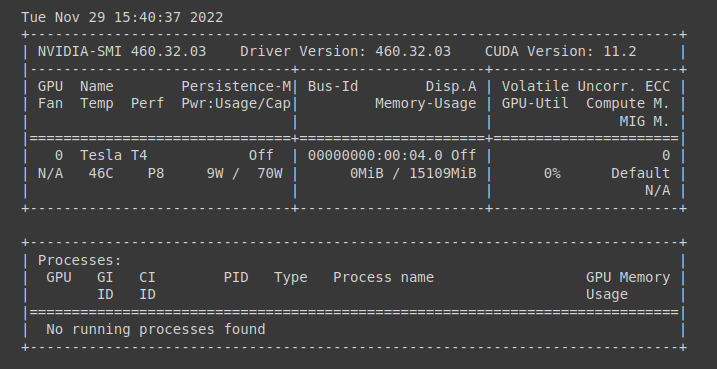
\includegraphics[scale=0.5]{nvidiasmi.png}
\end{center}


\subsubsection{Compilation and Execution}
Here, we use the tutorial proposed by \href{https://colab.research.google.com/github/ENCCS/OpenACC-CUDA-beginners/blob/colab_gcc/examples/openACC_CUDA_colab.ipynb#scrollTo=6WS9YBwSAsnf}{}\\
\textbf{Compilation flag}
To use the OpenACC directives, one should inform the compiler by adding the special flag. For the GNU compiler, the \code{-fopenacc} flag is required.\\
\textbf{Directives}
Inside the code source, the use of OpenACC directives allow to warn the compute regions that should be performed on the GPU device, and enable the GPU-acceleration.\\
\begin{mylisting}
#ifdef _OPENACC
	use openacc
#endif
\end{mylisting}


\subsubsection{Preview on the CPU code}
Before thinking about optimizing an application, one should first make a performance-profiling and find hotspots in the source code. In other words, the idea is to get information about the regions which take a significant percentage of the runtime.\\ 
Let's note that in Fortran language, considering a two dimensions array, the reading is made column by line. 

\subsubsection{OpenACC}
First, we could ask why using OpenACC rather than CUDA to port a GPU implementation. The reason is because OpenACC requires less rewriting of code and allow to keep the framework of the source code unchanged and maintain the sequential code.\\ 
Also, OpenACC is interoperable with CUDA, which means that later on, one could just add CUDA in some part of the code to adjust regarding some needing performance.\\
Most of what will be presented here comes from this \href{https://colab.research.google.com/github/ENCCS/OpenACC-CUDA-beginners/blob/colab_gcc/examples/openACC_CUDA_colab.ipynb}{tutorial}.\\
OpenACC is a directive-bases parallel programming approach used to accelerate in an easy way applications.\\
One of the limitations using Colab is the timeout of 90 minutes which means that the files uploaded to work with will not be available passing this time.
\begin{lstlisting}
!nvidia-smi
\end{lstlisting}

Here the outcome of this command:
\begin{center}
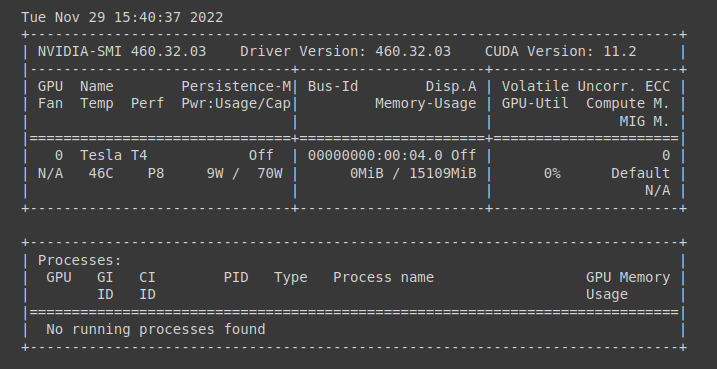
\includegraphics[scale=0.5]{nvidiasmi.png}
\end{center}

\subsubsection{OpenACC Syntax}
Only the Fortran syntax will be presented here, but one could easily find the C/C++ Syntax if working with these langages.\\
The directives are added to a serial code using the syntax:
\begin{mylisting}
!\$acc \textit{directive clauses}
<code>
\end{mylisting}
This syntax is formatted as comments and will be read only if we add the compiler flag \code{fopenacc} to enable OpenACC. If not enabled the directives will be treated as comment by the compiler.\\
These directives will allow to inform the compiler how to manage loop parallelization for the computing, but also to manage data transfer between CPU and GPU memory. The latter can be very time consuming as we will see later. \\
And finally, the \textbf{Clauses} are here attached to the directives for more specifications. 


\subsection{Porting to GPU using OpenACC}
In this section, we will use an existing program which perform a simple addition between two vectors.
\begin{mylisting}
program vectorsum
#ifdef _OPENACC
  use openacc
#endif
  implicit none
  integer, parameter :: rk = selected_real_kind(12)
  integer, parameter :: ik = selected_int_kind(9)
  integer, parameter :: nx = 102400

  real(kind=rk), dimension(nx) :: vecA, vecB, vecC
  real(kind=rk)    :: sum
  integer(kind=ik) :: i

  ! Initialization of vectors
  do i = 1, nx
     vecA(i) = 1.0_rk/(real(nx - i + 1, kind=rk))
     vecB(i) = vecA(i)**2
  end do

  ! Addition
  do i = 1, nx
     vecC(i) = vecA(i) + vecB(i)
  end do

  ! Compute the check value
  write(*,*) 'Reduction sum: ', sum(vecC)
  
end program vectorsum
\end{mylisting}

\subsubsection{Time profiling}
In most ressources, some powerful tools are used to perform a an analysis of the time consumption. These tools are part of the PGI compiler. In our case, we are using a GNU Fortran compiler, therefore, we opted for the use of the basic routines \code{cpu\_time} function to highlight the hotspots of our code.\\
A simple implementation of a routine can give us access to some relevant information ; also some instructions have been added to save them in an output file. The results look like:
\begin{center}
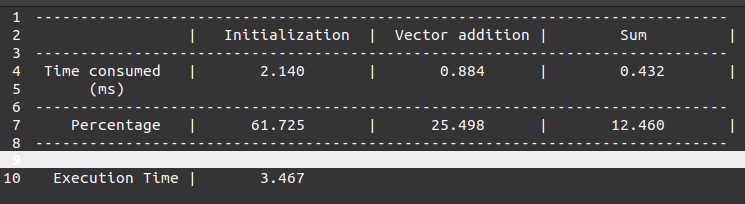
\includegraphics[scale=0.5]{serial_data.png}
\end{center}

\subsubsection{Loops parallelization}

\subsubsection{Data optimization}

\subsubsection{Loop optimization}


\subsection{Index}
\code{gang}: Depending the architecture, \code{gang} can have different meanings. On a multicore CPU, \code{gang} means generally a thread. As for a GPU, \code{gang} means a thread block. The idea behind it is that \code{gang} is the outer-most level of parallelism for any architecture.

\end{document}